\documentclass[TS,authoryear,toc]{lsstdoc}
\input{meta}

\usepackage{amsmath}
\usepackage{amssymb}
\usepackage{dsfont}
\usepackage{hyperref}

\hypersetup{
    colorlinks = true,
    allcolors = blue,
}

% Local commands go here.

%If you want glossaries
%\input{aglossary.tex}
%\makeglossaries

\title{Notes on Wavefront Estimation}

% Optional subtitle
% \setDocSubtitle{A subtitle}

\author{John Franklin Crenshaw}

\setDocRef{SITCOMTN-111}
\setDocUpstreamLocation{\url{https://github.com/lsst-sitcom/sitcomtn-111}}

\date{\vcsDate}

% Optional: name of the document's curator
% \setDocCurator{The Curator of this Document}

\setDocAbstract{%
The Rubin Observatory active optics system (AOS) uses the wavefront estimation pipeline (WEP) to estimate the wavefront of the telescope from out-of-focus images of stars. This note describes the theory behind and derives the equations used by the WEP.
}

% Change history defined here.
% Order: oldest first.
% Fields: VERSION, DATE, DESCRIPTION, OWNER NAME.
% See LPM-51 for version number policy.
\setDocChangeRecord{%
  \addtohist{1}{2024-02-13}{Initial version}{John Franklin Crenshaw}
}


\begin{document}

% Create the title page.
%\maketitle
\mkshorttitle
% Frequently for a technote we do not want a title page  uncomment this to remove the title page and changelog.
% use \mkshorttitle to remove the extra pages


\label{start}

The Rubin Observatory's Simonyi Survey Telescope must use an active optics system to correct perturbations to the optical alignment and mirror figures.
Achieving these corrections requires the following steps:
\begin{enumerate}
  \item estimating the wavefront of the optical system,
  \item using the wavefront to estimate the current configuration of the optical system,
  \item using the current optical configuration to derive forces to apply to the hexapods and actuators.
\end{enumerate}
This note concerns the first step, filling in details behind \citet{2015ApOpt..54.9045X} using the notation of version 9 of the wavefront estimation pipeline (WEP).

Estimating the wavefront typically requires an optical model for mapping the photons from the pupil to the image plane.
Deriving this mapping is the focus of Section~\ref{sec:mapping}.
Section~\ref{sec:estimation} discusses different methods for estimating the wavefront of the telescope from defocused images.


\section{Mapping from the Pupil to the Image Plane}
\label{sec:mapping}

\begin{figure}[t]
  \centering
  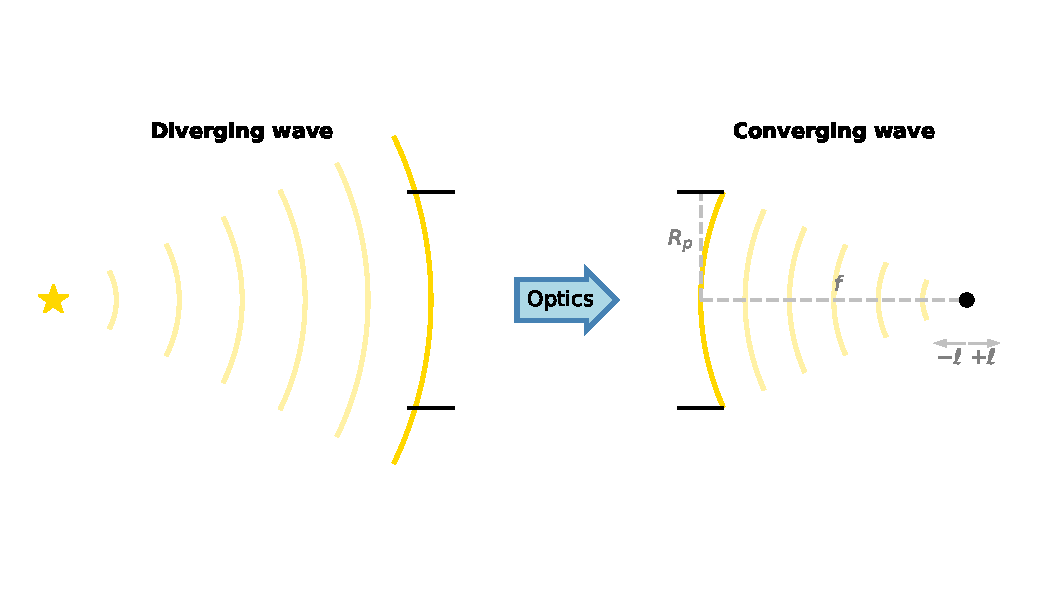
\includegraphics[width=0.9\linewidth]{figures/telescope_blackbox.pdf}
  \caption{
      Black box diagram of a telescope.
      An incoming diverging wave enters the pupil on the left, is transformed by the optical system, and is emitted from the pupil on the right, where it converges on the focal plane.
  }
  \label{fig:telescope}
\end{figure}

In this section we define the wavefront of the telescope and derive a mapping from photon positions on the pupil to the corresponding positions on the image plane.

The optical system of a telescope can be treated as a black box which receives an incoming wave on the pupil plane and converts that wave to one converging on the focal plane (Fig.~\ref{fig:telescope}).
For example, ignoring phase perturbations from e.g. atmospheric turbulence, we can assume the incoming wave is a plane wave with phase
\begin{align}
    \varphi(z, \mathbf{x}) = -k z,
\end{align}
where $k$ is the wavenumber and $\mathbf{x} = (x, y)$ is a 2D transverse position vector.
After passing through the optical system, the wave emerges with the phase
\begin{align}
    \varphi(z, \mathbf{x}) = -k \sqrt{(z - f)^2 + \mathbf{x}^2},
\end{align}
where $f$ is the focal length of the system and we have defined $z=0$ at the pupil.

We define the wavefront at the pupil using the reference sphere, which we define as the sphere with radius $f$ that is centered on the focal plane and tangent to the center of the pupil -- i.e., the first emerging wavefront on the right of Fig.~\ref{fig:telescope}.
The points on the reference sphere are the set
\begin{align}
  \left\{ 
    (z_p, \mathbf{x}_p) ~ \vert ~
    z_p = f - \sqrt{f^2 - \mathbf{x}_p^2}, ~~
    \mathbf{x}_p^2 < R_p^2
  \right\},
\end{align}
where $R_p$ is the radius of the pupil.

On the reference sphere the gradient of the phase is
\begin{align}
    \nabla \varphi(\mathbf{x}_p)
    = \frac{k}{f} \left( \sqrt{f^2 - \mathbf{x}_p^2} ~ \hat{\mathbf{z}} -\mathbf{x}_p \right).
    \label{eq:phase-gradient}
\end{align}
We have added the subscript $p$ to the transverse vector $x$ to remind that this equation applies to the wavefront at the pupil.
Recall that photons propagate in the direction of the phase gradient.
From Eq.~\ref{eq:phase-gradient}, you can see that a photon starting at $(z_p, \mathbf{x}_p)$ propagates in the direction $(f - z_p, -\mathbf{x}_p)$, and thus converges on the point $(f, 0)$.
In other words, all photons emerging from the pupil converge on the focal point.

The above assumes a perfect optical system.
We wish to consider an optical system with perturbations to alignment and mirror figure, which induce a phase perturbation $\delta \varphi = -k \, W(\mathbf{x}_p)$. $W(\mathbf{x}_p)$ is known as the optical path difference (OPD) and is defined on the reference sphere.
With this perturbation, the phase gradient is now
\begin{align}
    \nabla \varphi(\mathbf{x}_p)
    = \frac{k}{f} \left(\sqrt{f^2 - \mathbf{x}_p^2} ~ \hat{\mathbf{z}} -\mathbf{x}_p - f \nabla_\mathbf{x} W(\mathbf{x}_p) \right).
    \label{eq:phase-gradient-pert}
\end{align}
From Eq.~\ref{eq:phase-gradient-pert} you can see the effect of optical perturbations is to deflect photons from position $\mathbf{x}_p$ on the reference sphere by the amount $-f \nabla_\mathbf{x} W(\mathbf{x}_p)$ on the focal plane.

\begin{figure}[t]
    \centering
    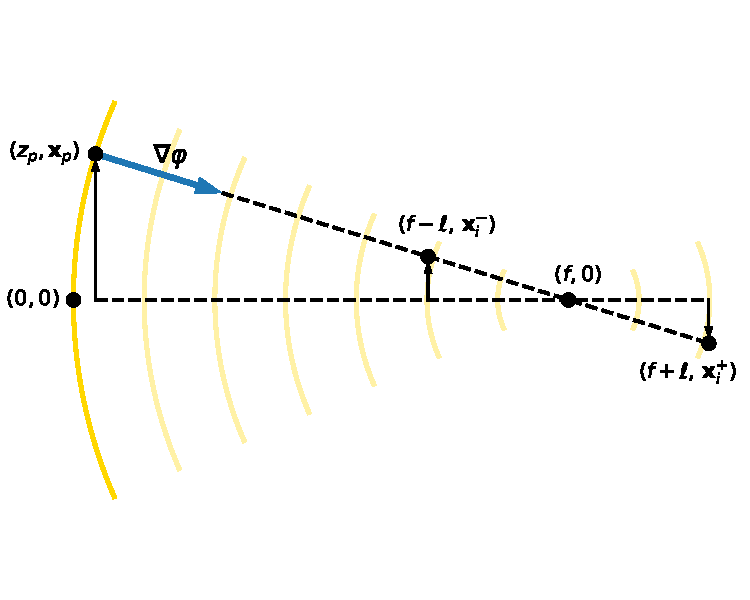
\includegraphics[width=0.6\linewidth]{figures/similar_triangles.pdf}
    \caption{
        Diagram showing the mapping of a pupil point to points on the defocused image planes.
        Note the line from $(z_p, \mathbf{x}_p)$ to $(f + \ell, \, \mathbf{x}_i^+)$ only passes through the focal point when $W(\mathbf{x}_p) = 0$.
        This geometry is the basis for Eq.~\ref{eq:triangles}.
    }
    \label{fig:triangles}
\end{figure}

Active optics systems usually operate on defocused images.
In particular, Rubin uses images from curvature wavefront sensors (CWFSs) that are offset on either side of the focal plane by a small distance $\ell$.
Thus we are interested in the images formed on the defocused planes at positions $z_i^\pm = f \pm \ell$.
We can determine the mapping from pupil position $\mathbf{x}_p$ to image position $(\mathbf{x}_i^\pm, z_i^\pm)$ using the similar triangles in Fig.~\ref{fig:triangles}:
\begin{align}
    \frac{
        \mathbf{x}_i^\pm - \mathbf{x}_p
    }{
        z_i^\pm - z_p
    } = \frac{
        \nabla_\mathbf{x} \varphi(\mathbf{x}_p)
    }{
        ~ \partial \varphi(\mathbf{x}_p) / \partial z ~
    }
    ~ \implies ~ 
    \frac{
        \mathbf{x}_i^\pm - \mathbf{x}_p
    }{
        \sqrt{f^2 - \mathbf{x}_p} \pm \ell
    } = 
    \frac{
        - \mathbf{x}_p - f \nabla_\mathbf{x} W(\mathbf{x}_p)
    }{
        \sqrt{f^2 - \mathbf{x}_p^2}
    }.
    \label{eq:triangles}
\end{align}
Solving for the image position yields
\begin{align}
    \mathbf{x}_i^\pm = \mp \frac{\ell}{\sqrt{f^2 - \mathbf{x}_p^2}} \, \mathbf{x}_p - f \left( 1 \pm \frac{\ell}{\sqrt{f^2 - \mathbf{x}_p^2}} \right) \nabla_\mathbf{x} W(\mathbf{x}_p).
    \label{eq:map-physical-full}
\end{align}
We see that for an unaberrated wavefront, the magnitude of the vector $\mathbf{x}_p$ shrinks linearly with respect to position on the $z$-axis.
The effect of defocused-imaging is to simply adjust the linear scaling according to the fraction of the $z$-axis distance to the focal plane at which the defocused plane lies (plus an inversion of the vector on the other side of focus).
The deflection due to the phase perturbation is similarly rescaled.
For typical configurations, however, the rescaling of the deflection term is very nearly one (for Rubin, the maximum deviation is only one part in ten thousand) and can therefore be safely neglected.
Thus we have
\begin{align}
    \mathbf{x}_i^\pm = \mp \frac{\ell}{\sqrt{f^2 - \mathbf{x}_p^2}} \mathbf{x}_p - f \nabla_\mathbf{x} W(\mathbf{x}_p).
    \label{eq:map-physical}
\end{align}

In the absence of wavefront perturbations, the radius of the pupil projected onto the defocused image plane is
\begin{align}
    R_i = \frac{\ell \, R_p}{\sqrt{f^2 - R_p^2}} = \frac{\ell}{\sqrt{4 N^2 - 1}},
\end{align}
where $N$ is the focal ratio (or $f$-number) of the telescope.
It is convenient to rewrite Eq.~\ref{eq:map-physical} in terms of the normalized, centered coordinates
\begin{align}
    \mathbf{u} = (u, v) &\equiv \frac{1}{R_p} \mathbf{x} \\
    \mathbf{u'} = (u', v') &\equiv \frac{1}{R_i} \Big[ \mathbf{x} + f \nabla_\mathbf{x} W(\mathbf{0}) \Big].
\end{align}
In these coordinates, the unaberrated pupil has a radius of $1$ on both the pupil and image planes, and the aberrated pupil is centered on both the pupil and image planes.
With these coordinate transformations, the mapping from pupil to image plane is
\begin{align}
    \mathbf{u'}_{\!i}^\pm = \mp \sqrt{\frac{4 N^2 - 1}{4 N^2 - \mathbf{u}_p^2}} \, \mathbf{u}_p - \frac{2 N \sqrt{4 N^2 - 1}}{\ell} \Big[ \nabla_\mathbf{u} W(\mathbf{u}_p) - \nabla_\mathbf{u} W(\mathbf{0}) \Big].
    \label{eq:map}
\end{align}
In the limit of $N \gg 1$, we have
\begin{align}
    \mathbf{u'}_{\!i}^\pm = \mp \mathbf{u}_p - \frac{4 N^2}{\ell} \Big[ \nabla_\mathbf{u} W(\mathbf{u}_p) - \nabla_\mathbf{u} W(\mathbf{0}) \Big],
    \label{eq:paraxial}
\end{align}
which matches Eq.'s~11 and 12 of \citet{1993JOSAA..10.2277R} (note this paper only explicitly derives formulae for the intrafocal image, they do not discard the negligible adjustment to the deflection term in Eq.~\ref{eq:map-physical-full}, and they do not center their rescaled coordinates).
For Rubin $N = 1.234$, so the $N \gg 1$ assumption cannot be made but Eq.~\ref{eq:paraxial} is included in WEP as the ``paraxial'' model for testing purposes.

Using the mapping from pupil to images planes we can predict the image intensity on the defocused planes.
Let $I(\mathbf{u}_p)$ be the intensity on the pupil (which for distant point sources is typically uniform) and $I'(\mathbf{u}'_i)$ be the intensity on the image plane.
From flux conservation,
\begin{align}
    I(\mathbf{u}_p) \, d \mathbf{u}_p = 
    I'(\mathbf{u}'_i) \, d \mathbf{u}'_i = 
    I'(\mathbf{u}'_i) \left\vert \frac{d \mathbf{u}'_i}{d \mathbf{u}_p} \right\vert d \mathbf{u}_p,
\end{align}
and therefore
\begin{align}
    I(\mathbf{u}_p) = I'(\mathbf{u}'_i) \left\vert \frac{d \mathbf{u}'_i}{d \mathbf{u}_p} \right\vert,
\end{align}
where $\vert d \mathbf{u}'_i / d \mathbf{u}_p \vert$ is the determinant of the Jacobian of the $\mathbf{u}_p \to \mathbf{u}'_i$ transformation.

The Jacobian is
\begin{align}
    \frac{d\mathbf{u'}_{\!i}^\pm}{d\mathbf{u}_p} = 
    \sqrt{\frac{4N^2 - 1}{4N^2 - \mathbf{u}_p^2}} \left[
        \mp \mathds{1}_2 + \frac{\mathbf{u}_p \otimes \mathbf{u}_p}{4N^2 - \mathbf{u}_p^2}
    \right] - \frac{2N \sqrt{4N^2 - 1}}{\ell} \frac{d^2 W(\mathbf{u}_p)}{d \mathbf{u}^2}.
    \label{eq:jacobian}
\end{align}
In particular, $\mathds{1}_2$ is the $2 \times 2$ identity matrix, the outer product is
\begin{align}
    \mathbf{u}_p \otimes \mathbf{u}_p = 
    \begin{pmatrix}
        u_p^2   & u_p v_p \\
        v_p u_p & v_p^2
    \end{pmatrix},
\end{align}
and $d^2 W(\mathbf{u}_p) / d \mathbf{u}^2$ is the Hessian matrix.
In the limit $N \gg 1$, this becomes
\begin{align}
    \frac{d\mathbf{u'}_{\!i}^\pm}{d\mathbf{u}_p} = \mp \mathds{1}_2 - \frac{4 N^2}{\ell} \frac{d^2 W(\mathbf{u}_p)}{d \mathbf{u}^2}.
\end{align}
the determinant of which matches Eq.~13 of \citet{1993JOSAA..10.2277R}.

Note that Eq.'s~\ref{eq:map}~and~\ref{eq:jacobian} reproduce Eq.'s~22-28 from \citet{2015ApOpt..54.9045X} if you take the definition of $m$ from the \texttt{CompensableImage} class in WEP version 8.

The equations above assume a wave that is converging on the center of the focal plane.
This is a poor assumption for wide field angles, for which we use a numerical model fit using \texttt{Batoid}.
In this model, we represent the OPD in a Zernike series:
\begin{align}
  W(\mathbf{u}_p) = \sum_i \alpha_i Z_i(\mathbf{u}_p),
  \quad \big[ \text{OPD Only} \big]
\end{align}
where the $\alpha_i$ are coefficients in meters (see Section~\ref{sec:estimation} for more details on Zernike polynomials).
A second series of coefficients fit by \texttt{Batoid}, $\beta_i$, are added to these coefficients such that
\begin{align}
  W(\mathbf{u}_p) = \sum_i (\alpha_i + \beta_i) Z_i(\mathbf{u}_p).
  \quad \big[ \text{OPD} + \texttt{Batoid}~\text{model} \big]
\end{align}
We then use the equations above, dispensing with any terms that do not directly reference $W(\mathbf{u}_p)$.
That is, 
\begin{align}
  \mathbf{u'}_{\!i}^\pm = - \frac{2 N \sqrt{4 N^2 - 1}}{\ell} \Big[ \nabla_\mathbf{u} W(\mathbf{u}_p) - \nabla_\mathbf{u} W(\mathbf{0}) \Big]
  \quad \text{and} \quad
  \frac{d\mathbf{u'}_{\!i}^\pm}{d\mathbf{u}_p} = - \frac{2N \sqrt{4N^2 - 1}}{\ell} \frac{d^2 W(\mathbf{u}_p)}{d \mathbf{u}^2}.
\end{align}
Note the Batoid coefficients only account for off-axis projection effects and do not account for the intrinsic aberrations associated with the telescope.


\section{Inferring the Wavefront from Defocused Images}
\label{sec:estimation}

The goal of the active optics system is to infer $W(\mathbf{u}_p)$, the OPD of the optical system, from the defocused image intensity $I_i(\mathbf{u}_i, z_i = f \pm \ell)$ using the relations derived in the previous section.
This is an inversion problem.
In the following subsections, I detail three different methods for performing this inversion.

In all cases, we seek to represent the OPD as a linear combination of annular Zernike polynomials defined on the pupil:
\begin{align}
    W(\mathbf{u}_p) = \sum_i \alpha_i Z_i(\mathbf{u}_p), 
\end{align}
where the coefficients $\alpha_i$ carry the units.
The annular Zernike polynomials are a complete orthogonal set of basis functions that roughly correspond to traditional optical aberrations.
We use the Noll index scheme -- i.e. $Z_4$ corresponds to defocus, $Z_5$ and $Z_6$ correspond to oblique and vertical astigmatism, etc.
We use the normalization
\begin{align}
    \iint Z_i(\mathbf{u}_p) Z_j(\mathbf{u}_p) \, d \mathbf{u}_p = A \delta_{ij},
    \label{eq:norm}
\end{align}
where $A$ is the pupil area.
Using the normalized coordinates defined in the previous section, $A = \pi (1 - \varepsilon^2)$ where $\varepsilon$ is the fractional obscuration of the pupil.
For Rubin this is $\varepsilon = 0.612$.

\subsection{Inversion via forward modeling}

One method for estimating the Zernike coefficients is to guess an initial set of coefficients and use the formulae from the previous section to forward model the image on one (or both) of the defocused plane(s).
You can then use an optimization routine to determine the set of Zernike coefficients that best matched the observed image.
This is the method proposed by \citet{janish2012} and implemented in the \texttt{Danish} algorithm.

In addition to optimizing the Zernike coefficients, \texttt{danish} also jointly optimizes a source pixel offset and the astronomical seeing.
The former allows \texttt{danish} to account for miscentering, while the latter accounts for the atmospheric turbulence that blurs any image taken with a ground based telescope.

\texttt{danish} also implements a mask model to account for vignetting which it also projects onto the image plane.
This is similar to the mask model from \citet{janish2012} which estimates the fractional illumination of pixels on the pupil edge by making a locally linear approximation of the circular pupil across each of the edge pixels.
However the projection of the pupil onto the image plane is only circular in the absence of wavefront aberrations.
\texttt{danish} improves on the model of \citet{janish2012}, therefore, by accounting for wavefront aberrations in the mask model.

Early testing suggests this method is prone to outliers, but is otherwise more accurate than the TIE (described below).
\texttt{danish} is also slower than the TIE.


\subsection{Inversion via Solving the Transport of Intensity Equation}

If you have a pair of images from both sides of focus, you can estimate the wavefront by solving the transport of intensity equation (TIE).
The advantage of the TIE over the forward modeling method is that it admits an algebraic solution which is faster than general optimization.
In reality the TIE must be iteratively solved to converge on the true wavefront, however even with these iterations the TIE method is typically faster than the forward modeling method.
The disadvantage is that the TIE method is complicated and more sensitive to issues such as miscentering, blending, and vignetting.

We start by deriving the TIE in Section~\ref{sec:tie-derivation}.
In Section~\ref{sec:approx-I-dIdz} we discuss approximations of the beam intensity and longitudinal derivative, which are key inputs to the TIE.
Finally, in Section~\ref{sec:exp} we discuss solving the TIE via Zernike expansion.


\subsubsection{Deriving the TIE}
\label{sec:tie-derivation}

We will derive the TIE by applying conservation of energy in the paraxial limit.
You can also derive the TIE as the imaginary part of the paraxial Helmholtz equation (i.e. the time-independent wave equation).
Note these paraxial assumptions concern the incoming photon beam, which for distant point sources is very nearly a plane wave.
This differs from the previous section in which we considered a photon beam after it had passed through the optical system.
In that case, the paraxial assumption is invalid for systems with low focal ratio, like the Rubin Observatory's Simonyi Survey Telescope. 

The complex amplitude of a monochromatic wave with intensity $I$ and phase $\varphi$ can be written
\begin{align}
    \Psi(z, \mathbf{x}) = \sqrt{I(z, \mathbf{x})} e^{i\varphi(z, \mathbf{x})}.
\end{align}
The phase of this wave can be expanded
\begin{align}
    \varphi(z, \mathbf{x}) = k_z z + \mathbf{k}_\mathbf{x} \cdot \mathbf{x},
\end{align}
where
\begin{align}
    k^2 = k_z^2 + |\mathbf{k}_\mathbf{x}|^2  = \left(\frac{2\pi}{\lambda}\right)^2,
\end{align}
and $\lambda$ is the wavelength of the light.

The Poynting vector is the energy flux of the wave.
By definition, the intensity is the magnitude of the time average of the Poynting vector: $|\langle \mathbf{S}(z, \mathbf{x}) \rangle| = I(z, \mathbf{x})$.
Since photons propagate perpendicular to the wavefront, the time average Poynting vector must also be proportional to the gradient of the phase: $\langle \mathbf{S}(z, \mathbf{x}) \rangle \propto \nabla \varphi(z, \mathbf{x})$.
Combining these two requirements, we have
\begin{align}
    \langle \mathbf{S}(z, \mathbf{x}) \rangle = \frac{1}{k} I(z, \mathbf{x}) \nabla \varphi(z, \mathbf{x}).
\end{align}

Now let's use the paraxial approximation.
That is, we consider a wave whose direction is very nearly aligned with the $z$ axis.
In this limit, $|\mathbf{k}_{x,y}| / k_z \ll 1$, and we can approximate $k_z \approx k$.
Then,
\begin{align}
    \nabla \varphi(z, \mathbf{x}) = k \hat{\mathbf{z}} + \nabla_\mathbf{x} \varphi(\mathbf{x}),
\end{align}
where $\nabla_\mathbf{x}$ is the transverse gradient and $\varphi(\mathbf{x})$ is the transverse component of the phase.
We can now write
\begin{align}
    \langle \mathbf{S}(\mathbf{x}, z) \rangle = 
    I(\mathbf{x}, z) \hat{\mathbf{z}} + \frac{1}{k} I(\mathbf{x}, z) \nabla_\mathbf{x} \varphi(\mathbf{x}).
\end{align}

Finally, we can apply conservation of energy.
In the vacuum, energy conservation demands that
\begin{align}
    \nabla \cdot \langle \mathbf{S}(z, \mathbf{x}) \rangle = 0.
\end{align}
Plugging in the time-averaged Poynting vector in the paraxial limit, we get the TIE:
\begin{align}
    \frac{\partial I(z, \mathbf{x})}{\partial z} + \nabla_\mathbf{x} \cdot \left[\,\frac{1}{k} \, I(z, \mathbf{x}) \nabla_\mathbf{x} \varphi(\mathbf{x})\right] = 0.
    \label{eq:tie-full}
\end{align}

The TIE has a simple interpretation in terms of conservation of energy.
In the paraxial limit, $I(z, \mathbf{x})$ is the energy flux in the longitudinal direction, and $k^{-1} I(z, \mathbf{x}) \nabla_\mathbf{x} \varphi(\mathbf{x})$ is the energy flux in the transverse direction.
The TIE says the decrease (increase) in longitudinal energy flux must be equal to the energy flux that is leaking out (coming in) the transverse direction.

We can see another obvious interpretation of the TIE if we use the fact that the pupil is uniformly illuminated by distant point sources --- i.e., $\nabla_\mathbf{x} I = 0$ inside the pupil.
Using this fact and applying our definition of the OPD yields
\begin{align}
    \nabla^2 W = \frac{1}{I} \frac{\partial I}{\partial z}.
\end{align}
In words, fractional changes in beam intensity are sourced by wavefront curvature. 

Finally, we can rewrite Eq.~\ref{eq:tie-full} in the normalized pupil coordinates of Section~\ref{sec:mapping}:
\begin{align}
    \frac{\partial I(0, \mathbf{u}_p)}{\partial z} = 
    \frac{1}{R^2} \nabla_\mathbf{u} \cdot [I(0, \mathbf{u}_p) \nabla_\mathbf{u} W(\mathbf{u}_p)].
\end{align}


\subsubsection{Approximating Beam Intensity and Longitudinal Derivative}
\label{sec:approx-I-dIdz}

To solve the TIE, we imagine that our defocused images are in-focus images of different cross sections of the photon beam.
We map the defocused images back to the pupil plane, but rather than thinking of the result as pupil illuminations, we imagine these are physical cross sections of the photon beam.
We can use the lens equation to determine the $z$ positions of these cross sections:
\begin{align}
    \frac{1}{o} + \frac{1}{f} = \frac{1}{i},
\end{align}
where $o$ and $i$ are the object and image positions, respectively.
We know our images are at locations $i = f \pm \ell$, so the objects are at locations
\begin{align}
    o = \mp \frac{f}{\ell}(f \pm \ell).
\end{align}
Thus, we see that the extrafocal image ($i = f + \ell$) correspond to a cross section of the beam before the exit pupil ($o<0$), while the intrafocal image ($i = f - \ell$) correspond to a cross section after the exit pupil ($o>0$).
For Rubin, $f \gg \ell$, and so we can state that $o \approx \mp \Delta z$, where
\begin{align}
    \Delta z = \frac{f^2}{\ell}.
\end{align}

With this knowledge in hand, we can make a linear approximation of $I$ and $\partial I / \partial z$:
\begin{align}
    I(0, \mathbf{u}_p) &\approx \frac{I(+\Delta z, \mathbf{u}_p) + I(-\Delta z, \mathbf{u}_p)}{2} \\[5pt]
    \frac{\partial I(0, \mathbf{u}_p)}{\partial z} &\approx \frac{I(+\Delta z, \mathbf{u}_p) - I(-\Delta z, \mathbf{u}_p)}{2\Delta z}.
\end{align}
Note this approximation is valid for small $\Delta z$.
Counter-intuitively, small values of $\Delta z$ correspond to large values of $\ell$.
For Rubin $\ell$ is quite small (meaning $\ell \ll f$) which violates this assumption.
Regardless, \citet{1993JOSAA..10.2277R} found that solving the TIE in the iterative manner described below converges to an accurate estimate of the wavefront.


\subsubsection{Solving via direct Zernike expansion}
\label{sec:exp}

With approximations of $I$ and $\partial I / \partial z$ in hand, we need to invert the TIE and solve for the OPD.
This can be done by expanding the OPD in a Zernike series:
\begin{align}
    \frac{\partial I(0, \mathbf{u}_p)}{\partial z} =
    \frac{1}{R^2} \sum_j \alpha_j
        \nabla_\mathbf{u} \cdot [I(0, \mathbf{u}_p) \nabla_\mathbf{u} Z_j(\mathbf{u}_p)].
\end{align}
We can then multiply each side by $Z_i(\mathbf{u}_p)$ and integrate over the pupil:
\begin{align}
    \iint Z_i(\mathbf{u}_p) \frac{\partial I(0, \mathbf{u}_p)}{\partial z} \, d\mathbf{u}_p =
    \frac{1}{R^2} \sum_j \alpha_j \, \iint Z_i(\mathbf{u}_p) \nabla_\mathbf{u} \cdot [I(0, \mathbf{u}_p) \nabla_\mathbf{u} Z_j(\mathbf{u}_p)] \, d\mathbf{u}_p.
\end{align}
Integrating by parts and using the fact that the beam intensity vanishes at the boundary yields
\begin{align}
    \iint Z_i(\mathbf{u}_p) \frac{\partial I(0, \mathbf{u}_p)}{\partial z} \, d\mathbf{u}_p =
    -\frac{1}{R^2} \sum_j \alpha_j \, \iint I(0, \mathbf{u}_p) \, \nabla_\mathbf{u} Z_i(\mathbf{u}_p) \cdot \nabla_\mathbf{u} Z_j(\mathbf{u}_p) \, d\mathbf{u}_p.
\end{align}
If we discretize the pupil into pixels indexed by $a, b$, the integrals become summations and the pixel size cancels, yielding
\begin{align}
    \sum_{a, b} ~ (Z_i)_{ab} \left(\frac{\partial I}{\partial z}\right)_{ab} =
    \sum_j \alpha_j \left[
        -\frac{1}{R^2} \sum_{ab} ~ I_{ab} \, (\nabla_\mathbf{u} Z_i \cdot \nabla_\mathbf{u} Z_j)_{ab}
    \right].
\end{align}
This is just a linear system.
If we define the vector
\begin{align}
    b_i = \sum_{a, b} ~ (Z_i)_{ab} \left(\frac{\partial I}{\partial z}\right)_{ab}
\end{align}
and the matrix
\begin{align}
    M_{ij} = -\frac{1}{R^2} \sum_{a,b} ~ I_{ab} \, (\nabla_\mathbf{u} Z_i \cdot \nabla_\mathbf{u} Z_j)_{ab},
\end{align}
then we seek to solve the equation
\begin{align}
    b_i = \sum_j M_{ij} \alpha_j.
\end{align}
Of course with real data there is no guarantee a solution exists.
Instead, we treat this as a regression problem and minimize the squared residuals of $b_i$.
In WEP this is done using \texttt{np.linalg.lstsq}.

Since both $b_i$ and $M_{ij}$ are constructed from the same pair of images, both are noisy and have correlated errors.
Therefore, you might expect an errors-in-variables model is needed for unbiased estimation of the $\alpha_i$.
However, a simple argument shows that the noise in $M_{ij}$ can be neglected and ordinary least squares is appropriate:
\begin{enumerate}
    \item The errors in $I$ and $\partial I / \partial z$ are of the same order of magnitude, and $R^2$ is $\mathcal{O}(10^2 \,\text{m})$.
    \item Due to the normalization condition (Eq.~\ref{eq:norm}), the values of $Z_i$ and $\nabla_\mathbf{u} Z_i$ are $\mathcal{O}(1)$.
    \item The errors in $M_{ij}$ are connected to the variables $b_i$ by the Zernike coefficients $\alpha_j$, which are  $\alpha_j \lesssim \mathcal{O}(10^{-6} \,\text{m})$ by assumption.
    \item Therefore the errors in $M_{ij}$ propagated to $b_i$ are roughly 8 orders of magnitude smaller than the errors native to $b_i$.
    
\end{enumerate}



\subsection{Inversion via Artificial Intelligence}
\label{sec:ai}

Rather than implementing the mapping equations of Section~\ref{sec:mapping} to solve for the wavefront, you can build a deep learning (or artificial intelligence; AI) network to implicitly learn the mapping by training the network to estimate Zernike coefficients directly from out-of-focus images.
For more details on this approach and comparisons to the TIE see \citet{2024AJ....167...86C}.




\appendix
% Include all the relevant bib files.
% https://lsst-texmf.lsst.io/lsstdoc.html#bibliographies
\section{References} \label{sec:bib}
\renewcommand{\refname}{} % Suppress default Bibliography section
\bibliography{local,lsst,lsst-dm,refs_ads,refs,books}

% Make sure lsst-texmf/bin/generateAcronyms.py is in your path
\section{Acronyms} \label{sec:acronyms}
\addtocounter{table}{-1}
\begin{longtable}{p{0.145\textwidth}p{0.8\textwidth}}\hline
\textbf{Acronym} & \textbf{Description}  \\\hline

AI & artificial intelligence \\\hline
CWFS & curvature wavefront sensor \\\hline
OPD & optical path difference \\\hline
TIE & transport of intensity equation \\\hline
WEP & wavefront estimation pipeline \\\hline
\end{longtable}

% If you want glossary uncomment below -- comment out the two lines above
%\printglossaries





\end{document}
